% Options for packages loaded elsewhere
\PassOptionsToPackage{unicode}{hyperref}
\PassOptionsToPackage{hyphens}{url}
%
\documentclass[
]{article}
\usepackage{lmodern}
\usepackage{amssymb,amsmath}
\usepackage{ifxetex,ifluatex}
\ifnum 0\ifxetex 1\fi\ifluatex 1\fi=0 % if pdftex
  \usepackage[T1]{fontenc}
  \usepackage[utf8]{inputenc}
  \usepackage{textcomp} % provide euro and other symbols
\else % if luatex or xetex
  \usepackage{unicode-math}
  \defaultfontfeatures{Scale=MatchLowercase}
  \defaultfontfeatures[\rmfamily]{Ligatures=TeX,Scale=1}
\fi
% Use upquote if available, for straight quotes in verbatim environments
\IfFileExists{upquote.sty}{\usepackage{upquote}}{}
\IfFileExists{microtype.sty}{% use microtype if available
  \usepackage[]{microtype}
  \UseMicrotypeSet[protrusion]{basicmath} % disable protrusion for tt fonts
}{}
\makeatletter
\@ifundefined{KOMAClassName}{% if non-KOMA class
  \IfFileExists{parskip.sty}{%
    \usepackage{parskip}
  }{% else
    \setlength{\parindent}{0pt}
    \setlength{\parskip}{6pt plus 2pt minus 1pt}}
}{% if KOMA class
  \KOMAoptions{parskip=half}}
\makeatother
\usepackage{xcolor}
\IfFileExists{xurl.sty}{\usepackage{xurl}}{} % add URL line breaks if available
\IfFileExists{bookmark.sty}{\usepackage{bookmark}}{\usepackage{hyperref}}
\hypersetup{
  pdftitle={ReporteKmeansOnline},
  pdfauthor={Jessic Vega},
  hidelinks,
  pdfcreator={LaTeX via pandoc}}
\urlstyle{same} % disable monospaced font for URLs
\usepackage[margin=1in]{geometry}
\usepackage{color}
\usepackage{fancyvrb}
\newcommand{\VerbBar}{|}
\newcommand{\VERB}{\Verb[commandchars=\\\{\}]}
\DefineVerbatimEnvironment{Highlighting}{Verbatim}{commandchars=\\\{\}}
% Add ',fontsize=\small' for more characters per line
\usepackage{framed}
\definecolor{shadecolor}{RGB}{248,248,248}
\newenvironment{Shaded}{\begin{snugshade}}{\end{snugshade}}
\newcommand{\AlertTok}[1]{\textcolor[rgb]{0.94,0.16,0.16}{#1}}
\newcommand{\AnnotationTok}[1]{\textcolor[rgb]{0.56,0.35,0.01}{\textbf{\textit{#1}}}}
\newcommand{\AttributeTok}[1]{\textcolor[rgb]{0.77,0.63,0.00}{#1}}
\newcommand{\BaseNTok}[1]{\textcolor[rgb]{0.00,0.00,0.81}{#1}}
\newcommand{\BuiltInTok}[1]{#1}
\newcommand{\CharTok}[1]{\textcolor[rgb]{0.31,0.60,0.02}{#1}}
\newcommand{\CommentTok}[1]{\textcolor[rgb]{0.56,0.35,0.01}{\textit{#1}}}
\newcommand{\CommentVarTok}[1]{\textcolor[rgb]{0.56,0.35,0.01}{\textbf{\textit{#1}}}}
\newcommand{\ConstantTok}[1]{\textcolor[rgb]{0.00,0.00,0.00}{#1}}
\newcommand{\ControlFlowTok}[1]{\textcolor[rgb]{0.13,0.29,0.53}{\textbf{#1}}}
\newcommand{\DataTypeTok}[1]{\textcolor[rgb]{0.13,0.29,0.53}{#1}}
\newcommand{\DecValTok}[1]{\textcolor[rgb]{0.00,0.00,0.81}{#1}}
\newcommand{\DocumentationTok}[1]{\textcolor[rgb]{0.56,0.35,0.01}{\textbf{\textit{#1}}}}
\newcommand{\ErrorTok}[1]{\textcolor[rgb]{0.64,0.00,0.00}{\textbf{#1}}}
\newcommand{\ExtensionTok}[1]{#1}
\newcommand{\FloatTok}[1]{\textcolor[rgb]{0.00,0.00,0.81}{#1}}
\newcommand{\FunctionTok}[1]{\textcolor[rgb]{0.00,0.00,0.00}{#1}}
\newcommand{\ImportTok}[1]{#1}
\newcommand{\InformationTok}[1]{\textcolor[rgb]{0.56,0.35,0.01}{\textbf{\textit{#1}}}}
\newcommand{\KeywordTok}[1]{\textcolor[rgb]{0.13,0.29,0.53}{\textbf{#1}}}
\newcommand{\NormalTok}[1]{#1}
\newcommand{\OperatorTok}[1]{\textcolor[rgb]{0.81,0.36,0.00}{\textbf{#1}}}
\newcommand{\OtherTok}[1]{\textcolor[rgb]{0.56,0.35,0.01}{#1}}
\newcommand{\PreprocessorTok}[1]{\textcolor[rgb]{0.56,0.35,0.01}{\textit{#1}}}
\newcommand{\RegionMarkerTok}[1]{#1}
\newcommand{\SpecialCharTok}[1]{\textcolor[rgb]{0.00,0.00,0.00}{#1}}
\newcommand{\SpecialStringTok}[1]{\textcolor[rgb]{0.31,0.60,0.02}{#1}}
\newcommand{\StringTok}[1]{\textcolor[rgb]{0.31,0.60,0.02}{#1}}
\newcommand{\VariableTok}[1]{\textcolor[rgb]{0.00,0.00,0.00}{#1}}
\newcommand{\VerbatimStringTok}[1]{\textcolor[rgb]{0.31,0.60,0.02}{#1}}
\newcommand{\WarningTok}[1]{\textcolor[rgb]{0.56,0.35,0.01}{\textbf{\textit{#1}}}}
\usepackage{graphicx,grffile}
\makeatletter
\def\maxwidth{\ifdim\Gin@nat@width>\linewidth\linewidth\else\Gin@nat@width\fi}
\def\maxheight{\ifdim\Gin@nat@height>\textheight\textheight\else\Gin@nat@height\fi}
\makeatother
% Scale images if necessary, so that they will not overflow the page
% margins by default, and it is still possible to overwrite the defaults
% using explicit options in \includegraphics[width, height, ...]{}
\setkeys{Gin}{width=\maxwidth,height=\maxheight,keepaspectratio}
% Set default figure placement to htbp
\makeatletter
\def\fps@figure{htbp}
\makeatother
\setlength{\emergencystretch}{3em} % prevent overfull lines
\providecommand{\tightlist}{%
  \setlength{\itemsep}{0pt}\setlength{\parskip}{0pt}}
\setcounter{secnumdepth}{-\maxdimen} % remove section numbering

\title{ReporteKmeansOnline}
\author{Jessic Vega}
\date{31/8/2020}

\begin{document}
\maketitle

\hypertarget{explicar-la-elecciuxf3n-del-nuxfamero-de-clusters-gruxe1fica-si-es-necesario}{%
\subsection{1) Explicar la elección del número de clusters (gráfica si
es
necesario)}\label{explicar-la-elecciuxf3n-del-nuxfamero-de-clusters-gruxe1fica-si-es-necesario}}

Con base en nuestra implementación del algoritmo de kmeans online,
elegimos el número de clusters como aquel que minimice la distancia
intra clusters (lo cual sabemos que es equivalente a maximizar la
distancia entre clusters).

En la gráfica siguiente podemos ver que conforme se incrementa el número
de clusters la distancia intra clusters disminuye, sin embargo por el
criterio de codo, elegimos 25 como un número de clusters prudente.

\begin{Shaded}
\begin{Highlighting}[]
\NormalTok{data <-}\StringTok{ }\KeywordTok{read.csv}\NormalTok{(}\DataTypeTok{file =} \StringTok{'docword.nips.txt'}\NormalTok{, }\DataTypeTok{header =} \OtherTok{FALSE}\NormalTok{, }\DataTypeTok{sep=}\StringTok{' '}\NormalTok{, }\DataTypeTok{skip =} \DecValTok{3}\NormalTok{)}
\KeywordTok{names}\NormalTok{(data) <-}\StringTok{ }\KeywordTok{c}\NormalTok{(}\StringTok{'Id.Doc'}\NormalTok{, }\StringTok{'Id.Word'}\NormalTok{, }\StringTok{'freq'}\NormalTok{)}
\KeywordTok{require}\NormalTok{(reshape2)}
\end{Highlighting}
\end{Shaded}

\begin{verbatim}
## Loading required package: reshape2
\end{verbatim}

\begin{Shaded}
\begin{Highlighting}[]
\NormalTok{docs.vector <-}\StringTok{ }\KeywordTok{dcast}\NormalTok{(data, Id.Doc }\OperatorTok{~}\NormalTok{Id.Word, }\DataTypeTok{value.var =} \StringTok{'freq'}\NormalTok{, }\DataTypeTok{fill=}\DecValTok{0}\NormalTok{)}
\NormalTok{docs.vector}\OperatorTok{$}\NormalTok{Id.Doc <-}\StringTok{ }\OtherTok{NULL}
\CommentTok{#docs.vector <- head(docs.vector, 100)}
\CommentTok{#docs.vector[, 1:dim(docs.vector)[2]] <- scale(docs.vector)}

\NormalTok{cluster <-}\StringTok{ }\DecValTok{1}\OperatorTok{:}\DecValTok{7}
\ControlFlowTok{for}\NormalTok{( i }\ControlFlowTok{in} \DecValTok{1}\OperatorTok{:}\DecValTok{7}\NormalTok{)}
\NormalTok{\{}
  \CommentTok{#print(i)}
\NormalTok{  res <-}\StringTok{ }\KeywordTok{kmeans.online.b}\NormalTok{(}\DataTypeTok{k=}\DecValTok{5}\OperatorTok{*}\NormalTok{i)}
\NormalTok{  cluster[i] <-}\StringTok{ }\KeywordTok{sum}\NormalTok{(res}\OperatorTok{$}\NormalTok{statas.intra)}
  \CommentTok{#print(cluster)}
\NormalTok{\}}
\KeywordTok{plot}\NormalTok{((cluster),}\DataTypeTok{type =} \StringTok{'l'}\NormalTok{, }\DataTypeTok{xlab =} \StringTok{'Multiplos de 5'}\NormalTok{, }\DataTypeTok{ylab =} \StringTok{'Var intra cluster'}\NormalTok{)}
\end{Highlighting}
\end{Shaded}

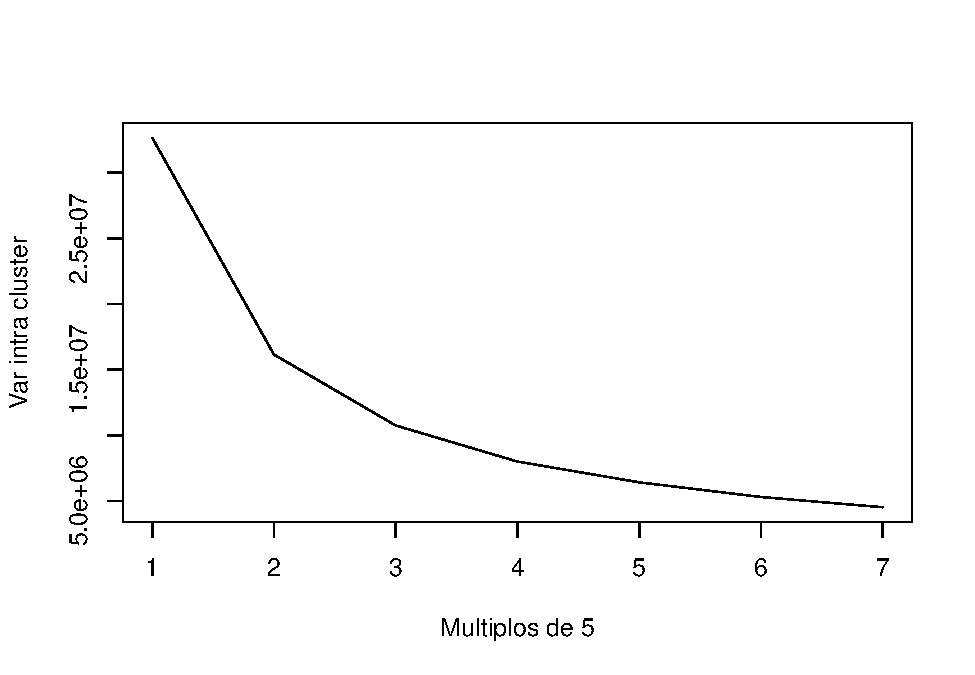
\includegraphics{ReporteKmeansOnlineJessVega_files/figure-latex/q1-1.pdf}

\begin{Shaded}
\begin{Highlighting}[]
\KeywordTok{plot}\NormalTok{(}\KeywordTok{abs}\NormalTok{(}\KeywordTok{diff}\NormalTok{(cluster)),}\DataTypeTok{type =} \StringTok{'l'}\NormalTok{,  }\DataTypeTok{xlab =} \StringTok{'Multiplos de 5'}\NormalTok{, }\DataTypeTok{ylab =} \StringTok{'diff(Var) intra cluster'}\NormalTok{)}
\end{Highlighting}
\end{Shaded}

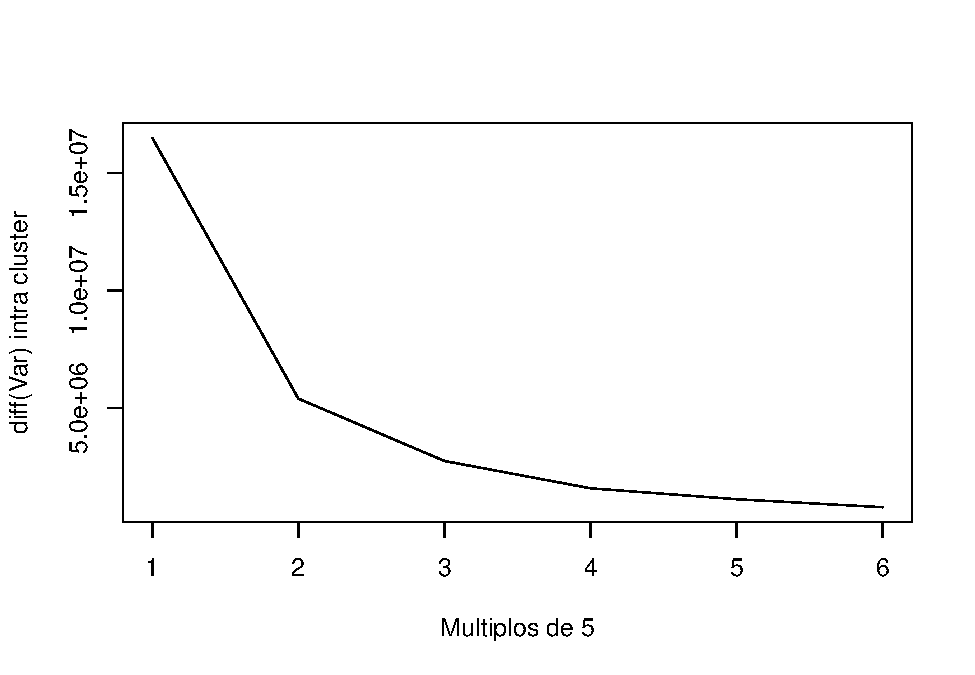
\includegraphics{ReporteKmeansOnlineJessVega_files/figure-latex/q1-2.pdf}

\hypertarget{mostrar-las-10-palabras-muxe1s-comunes-de-cada-cluster-en-una-tabla.}{%
\subsection{2) Mostrar las 10 palabras más comunes de cada cluster en
una
Tabla.}\label{mostrar-las-10-palabras-muxe1s-comunes-de-cada-cluster-en-una-tabla.}}

\begin{Shaded}
\begin{Highlighting}[]
\NormalTok{k <-}\StringTok{ }\DecValTok{25}
\NormalTok{res <-}\StringTok{ }\KeywordTok{kmeans.online.b}\NormalTok{(}\DataTypeTok{k=}\NormalTok{k)}
\NormalTok{words <-}\StringTok{ }\KeywordTok{read.csv}\NormalTok{(}\StringTok{'vocab.nips.txt'}\NormalTok{, }\DataTypeTok{header =} \OtherTok{FALSE}\NormalTok{)}
\KeywordTok{names}\NormalTok{(words) <-}\StringTok{ 'Palabra'}
\NormalTok{words}\OperatorTok{$}\NormalTok{Id.Word <-}\StringTok{ }\KeywordTok{as.numeric}\NormalTok{(}\KeywordTok{row.names}\NormalTok{(words))}
\NormalTok{data <-}\StringTok{ }\KeywordTok{merge}\NormalTok{(data, words, }\DataTypeTok{all.x=}\OtherTok{TRUE}\NormalTok{)}
\NormalTok{cluster.palabras.top10 <-}\StringTok{ }\KeywordTok{data.frame}\NormalTok{(}\DataTypeTok{Cluster=}\DecValTok{1}\OperatorTok{:}\DecValTok{25}\NormalTok{, }\DataTypeTok{Palabras=}\StringTok{''}\NormalTok{)}
\KeywordTok{require}\NormalTok{(dplyr)}
\end{Highlighting}
\end{Shaded}

\begin{verbatim}
## Loading required package: dplyr
\end{verbatim}

\begin{verbatim}
## 
## Attaching package: 'dplyr'
\end{verbatim}

\begin{verbatim}
## The following objects are masked from 'package:stats':
## 
##     filter, lag
\end{verbatim}

\begin{verbatim}
## The following objects are masked from 'package:base':
## 
##     intersect, setdiff, setequal, union
\end{verbatim}

\begin{Shaded}
\begin{Highlighting}[]
\ControlFlowTok{for}\NormalTok{ (i }\ControlFlowTok{in} \DecValTok{1}\OperatorTok{:}\DecValTok{25}\NormalTok{)}
\NormalTok{\{}
\NormalTok{  index <-}\StringTok{ }\KeywordTok{which}\NormalTok{(res}\OperatorTok{$}\NormalTok{tabla.master}\OperatorTok{$}\NormalTok{Cluster}\OperatorTok{==}\NormalTok{i)}
\NormalTok{  data.subset <-}\StringTok{ }\KeywordTok{subset}\NormalTok{(data, Id.Doc }\OperatorTok\StringTok{ }\NormalTok{index)}
\NormalTok{  data.subset }\OperatorTok\StringTok{ }\KeywordTok{select}\NormalTok{(Id.Doc, freq, Palabra) }\OperatorTok\StringTok{ }\KeywordTok{group_by}\NormalTok{(Palabra) }\OperatorTok\StringTok{ }\KeywordTok{summarise}\NormalTok{(}\DataTypeTok{freq=}\KeywordTok{sum}\NormalTok{(freq)) }\OperatorTok\StringTok{ }
\StringTok{    }\KeywordTok{arrange}\NormalTok{(}\OperatorTok{-}\NormalTok{freq) }\OperatorTok\StringTok{ }\KeywordTok{head}\NormalTok{(}\DecValTok{10}\NormalTok{) ->}\StringTok{ }\NormalTok{temp}
\NormalTok{  string <-}\StringTok{ }\KeywordTok{paste0}\NormalTok{(temp}\OperatorTok{$}\NormalTok{Palabra, }\DataTypeTok{collapse =} \StringTok{''}\NormalTok{, }\DataTypeTok{sep=}\StringTok{', '}\NormalTok{)}
\NormalTok{  cluster.palabras.top10}\OperatorTok{$}\NormalTok{Palabras[i] <-}\StringTok{ }\NormalTok{string}
\NormalTok{\}}
\end{Highlighting}
\end{Shaded}

\begin{verbatim}
## `summarise()` ungrouping output (override with `.groups` argument)
\end{verbatim}

\begin{verbatim}
## `summarise()` ungrouping output (override with `.groups` argument)
## `summarise()` ungrouping output (override with `.groups` argument)
## `summarise()` ungrouping output (override with `.groups` argument)
## `summarise()` ungrouping output (override with `.groups` argument)
## `summarise()` ungrouping output (override with `.groups` argument)
## `summarise()` ungrouping output (override with `.groups` argument)
## `summarise()` ungrouping output (override with `.groups` argument)
## `summarise()` ungrouping output (override with `.groups` argument)
## `summarise()` ungrouping output (override with `.groups` argument)
## `summarise()` ungrouping output (override with `.groups` argument)
## `summarise()` ungrouping output (override with `.groups` argument)
## `summarise()` ungrouping output (override with `.groups` argument)
## `summarise()` ungrouping output (override with `.groups` argument)
## `summarise()` ungrouping output (override with `.groups` argument)
## `summarise()` ungrouping output (override with `.groups` argument)
## `summarise()` ungrouping output (override with `.groups` argument)
## `summarise()` ungrouping output (override with `.groups` argument)
## `summarise()` ungrouping output (override with `.groups` argument)
## `summarise()` ungrouping output (override with `.groups` argument)
## `summarise()` ungrouping output (override with `.groups` argument)
## `summarise()` ungrouping output (override with `.groups` argument)
## `summarise()` ungrouping output (override with `.groups` argument)
## `summarise()` ungrouping output (override with `.groups` argument)
## `summarise()` ungrouping output (override with `.groups` argument)
\end{verbatim}

\begin{Shaded}
\begin{Highlighting}[]
\KeywordTok{write.csv}\NormalTok{(res}\OperatorTok{$}\NormalTok{tabla.master,}\DataTypeTok{file=}\StringTok{'tabla.master.csv'}\NormalTok{, }\DataTypeTok{row.names =} \OtherTok{FALSE}\NormalTok{)}
\NormalTok{cluster.palabras.top10}
\end{Highlighting}
\end{Shaded}

\begin{verbatim}
##    Cluster
## 1        1
## 2        2
## 3        3
## 4        4
## 5        5
## 6        6
## 7        7
## 8        8
## 9        9
## 10      10
## 11      11
## 12      12
## 13      13
## 14      14
## 15      15
## 16      16
## 17      17
## 18      18
## 19      19
## 20      20
## 21      21
## 22      22
## 23      23
## 24      24
## 25      25
##                                                                                    Palabras
## 1     network, unit, neural, system, learning, function, algorithm, error, hidden, weight, 
## 2    network, model, neural, learning, neuron, input, algorithm, function, system, output, 
## 3             network, unit, function, input, model, neural, output, training, layer, set, 
## 4  model, function, data, set, network, distribution, learning, vector, neural, algorithm, 
## 5       network, unit, neural, input, learning, function, output, weight, system, problem, 
## 6      function, model, algorithm, input, network, learning, set, neural, vector, problem, 
## 7        network, learning, weight, function, algorithm, input, neural, set, data, output, 
## 8        model, network, algorithm, learning, data, unit, hidden, function, set, training, 
## 9     network, neural, training, set, input, classifier, system, data, algorithm, problem, 
## 10        function, data, system, network, algorithm, set, neural, model, neuron, problem, 
## 11   learning, action, system, control, function, model, task, algorithm, network, result, 
## 12           network, learning, training, error, set, model, data, unit, input, algorithm, 
## 13            model, cell, network, data, input, motion, neural, learning, system, visual, 
## 14     learning, algorithm, function, model, set, vector, data, system, problem, training, 
## 15         network, neuron, neural, learning, input, model, set, pattern, function, error, 
## 16       cell, learning, network, algorithm, input, model, vector, output, system, weight, 
## 17        network, unit, input, output, layer, hidden, learning, set, algorithm, function, 
## 18             model, data, set, cell, function, point, network, input, parameter, number, 
## 19   learning, model, function, network, neuron, system, input, neural, object, algorithm, 
## 20          network, input, neural, algorithm, set, system, function, point, output, data, 
## 21           network, function, model, data, set, training, input, weight, method, neural, 
## 22          model, network, system, neural, input, neuron, data, cell, information, field, 
## 23           network, model, input, error, object, training, set, function, neural, image, 
## 24          network, system, function, point, error, input, learning, unit, model, neural, 
## 25           network, input, neural, model, set, system, training, data, learning, output,
\end{verbatim}

\begin{Shaded}
\begin{Highlighting}[]
\KeywordTok{require}\NormalTok{(xtable)}
\end{Highlighting}
\end{Shaded}

\begin{verbatim}
## Loading required package: xtable
\end{verbatim}

\hypertarget{breve-intuiciuxf3n-acerca-del-tipo-de-documento-que-cada-cluster-representa.}{%
\subsection{3) Breve intuición acerca del tipo de documento que cada
cluster
representa.}\label{breve-intuiciuxf3n-acerca-del-tipo-de-documento-que-cada-cluster-representa.}}

A grandes rasgos podemos englobar a los clusters en 4 meta clusters,
hacemos hincapié en que nuestra implementación puede, por ejemplo, estar
detectando papers (documentos) en años parecidos en lugar de grandes
temas que se distribuyen en el contenido de los mismos.

El primer meta cluster corresponde a papers de contenido meramente
teórico que no hace referencia a la aplicación de un método en
particular ni de su implementación por ello las palabras `algorithm',
`input' , `output', etc. no aparecen en su top 10. Este meta cluster
está integrado por los clusters: 1, 8, 10, 11, 20, 21 y 24.

El segundo meta cluster está formado por pares que hacen referencia a
implementaciones de métodos por lo cual contienen pseudocódigos y las
palabras `algorithm', `input' , `output' están presentes en ellos (en su
top 10). Ese meta cluster está formado por los clusters: 2, 3, 4, 5, 6,
7, 9, 12, 15 y 17.

El tercer meta cluster está formado por los papers de aplicación no
médica en donde se utiliza un conjunto de datos y se cuantifica el error
de una o varias técnicas de aprendizaje máquina. Este mega cluster está
formado por los clusters: 14, 18, 19 y 25

El último cluster se forma por los papers de aplicación médica, los
cuales se distinguen por las palabras `cell', `data' e `image'. Está
formado por los clusters: 13, 16, 22 y 23.

\hypertarget{cuxf3digo-del-algoritmo-solamente-la-secciuxf3n-donde-se-realiza-el-algoritmo-k-means.}{%
\subsection{4) Código del algoritmo: solamente la sección donde se
realiza el algoritmo
k-means.}\label{cuxf3digo-del-algoritmo-solamente-la-secciuxf3n-donde-se-realiza-el-algoritmo-k-means.}}

Se anexa en el archivo `KmeansOnlineJessVega.R'

\end{document}
